\documentclass[
% opciók nélkül: egyoldalas nyomtatás, elektronikus verzió
% twoside,     % kétoldalas nyomtatás
% tocnopagenum,% oldalszámozás a tartalomjegyzék után kezdődik
]{thesis-ekf}
\usepackage[T1]{fontenc}
\PassOptionsToPackage{defaults=hu-min}{magyar.ldf}
\usepackage[magyar]{babel}
\usepackage{mathtools,amssymb,amsthm}
\footnotestyle{rule=fourth}

\newtheorem{tetel}{Tétel}[chapter]
\theoremstyle{definition}
\newtheorem{definicio}[tetel]{Definíció}
\theoremstyle{remark}
\newtheorem{megjegyzes}[tetel]{Megjegyzés}

\begin{document}
\institute{Matematikai és Informatikai Intézet}
\title{Webfejlesztés modern technológiákkal}
\author{Vereczki Bálint Zoltán\\Programtervező Informatikus BSc}
\supervisor{Balla Tamás\\tanársegéd}
\city{Eger}
\date{2021}
\maketitle
\tableofcontents

\chapter*{Bevezetés}
Életünkben egyre nagyobb területén van jelen az internet. Bárhol, bármikor hozzáférhetünk a zsebünkben hordott mobilkészülékünkről, pár érintés után elérhetjük a legfrissebb információkat és híreket. Terméket és ételt rendelünk, tájékozódunk, hivatalos ügyeket intézünk, kapcsolatot tartunk, zenét és filmet nézünk, mindezt a világhálón. Ezen tevékenységek révén egyre interaktívabb weboldalak készültek az évek során, melyek ki tudják szolgálni ezeket az igényeket.

Kezdetben a weboldalak csupán statikus tartalommal rendelkeztek, melyhez (akárcsak ma) a HTML leírónyelvet és CSS stíluslapot használták. A JavaScript, majd később az AJAX megjelenése adott teret a dinamikus weboldalak elterjedésének.

A JavaScript a kliensoldalon történő DOM manipuláláson és eseménykezelésen kívül alkalmas webalkalmazások készítésére, illetve már szerveroldali programok írására is.

A felsőoktatásban elsődlegesen preferált kommunikációs forma a személyes konzultáción kívül az email. A legtöbb ügyintézés emailes levelezéssel történik, ez pedig egyes esetekben problémákhoz vezethet. A rengeteg üzenet között előfordul, hogy egy-egy fontos üzenet elkerüli a figyelmet. A jelenlegi járványhelyzet akadályozza a személyes beszélgetés lehetőségét, így csupán az online kommunikációra hagyatkozhatunk.

A szakdolgozatom célja ezen okoknál fogva egy olyan webes platform létrehozása, amely mind az oktatók, mind a hallgatók munkáját nagyban megkönnyíti és elősegíti. Lehetőséget nyújt a hallgatók, szakdolgozatok, konzultációs időpontok menedzselésére, határidőre megadott feladatok kiírására és azokon keresztül való visszajelzésre.

Szakdolgozatomban kitérek a webre, mint platformra és a használható architektúrákra, amiből az alkalmazást tekintve legmegfelelőbbet kiválasztom. Ezt követően áttekintem a lehetséges programozási nyelveket és keretrendszereket különös tekintettel kitérve a JavaScript által nyújtott megoldásokra.

\chapter{Téma elméleti kifejtése}
% https://developer.mozilla.org/en-US/docs/Learn/Server-side/First_steps/Introduction
% https://developer.mozilla.org/en-US/docs/Learn/Server-side/First_steps/Client-Server_overview
% https://developer.mozilla.org/en-US/docs/Learn/Getting_started_with_the_web/How_the_Web_works
% https://developer.mozilla.org/en-US/docs/Web/HTTP
% https://www.tutorialspoint.com/internet_technologies/internet_protocols.htm
\section{A web, mint platform}
Az egész világot behálózó számítógépes hálózatot internetnek nevezzük. Az internetre kapcsolódó számítógépek a TCP/IP (Transmission Control Procotol / Internet Protocol) segítségével képesek az egymással való kommunikációra. Minden egyes csatlakozott eszköz egy egyedi azonosítót kap, amelyet IP címnek nevezünk.
A weboldalakat az IP címek helyett könnyebben megjegyezhető domain címek alapján látogatjuk meg (pl. \emph{www.google.com}). Az internetre kapcsolódnak speciális szerverek is, mint például a DNS azaz névszerverek. Ennek a feladata az, hogy amikor a felhasználó elnavigál egy bizonyos domain címre, akkor azt lefordítsa a hozzá tartozó IP címre.

A fent említett protokollokon kívül számos jelentős protokoll létezik, melyeket más célokra tudunk használni. Ilyenek például:
\begin{itemize}
	\item UDP (User Datagram Protocol)
	\item FTP (File Transfer Protocol)
	\item SSH (Secure Shell)
	\item \emph{HTTP} (Hypertext Transfer Protocol)
\end{itemize}

Az internet által használt TCP (angolul Transmission Control Protocol) egy megbízható, kapcsolatorientált, végpont-végpont közötti kétirányú adatfolyamot biztosító protokoll. Megbízhatósága onnan ered, hogy az adatfolyam küldése közben nyugtázással biztosítja az adat megérkezését, hiba esetén pedig újrapróbálkozik az adat továbbításával.

Az UDP protokoll úgynevezett datagram alapon szállítja az adatot. A datagramban tárolódik a forrásport, célport, adat hossza, az ellenőrzőösszeg és maga a küldeni kívánt adat. Ellentétben a TCP-vel, nem biztosítja az üzenet megérkezését, olyan esetekben optimális a használata ahol a gyorsaság fontosabb tényező a megbízhatóságnál.

Az FTP állományok számítógépek közötti átvitelére használatos protokoll, melyhez két csatornát használ. Amikor a kliens csatlakozik az FTP szerverhez mindkét oldalon kiépül a vezérlő csatorna (angolul Control Process), melyen keresztül a kliens parancsokat adhat a távoli gépnek. Amint állományátviteli kérést adunk ki, kiépül az adatcsatorna, amin keresztül az adatcsere folyamata zajlik. 

% https://www.ssh.com/ssh/protocol/
Az FTP protokoll autentikáció szempontjából nem tekinthető biztonságosnak, ugyanis nem támogatja sem a TLS (angolul Transport Layer Security), sem az SSL (angolul Secure Sockets Layer) titkosítási protokollokat, a bejelentkezéshez használt felhasználónév és jelszó titkosítás nélkül kerül küldésre a klienstől a szerverig. Ezen probléma megoldásaként nyújt alternatívát az SSH (angolul Secure Shell) protokoll, amely biztonságos kapcsolatot épít ki a helyi és távoli számítógép között, és állományátvitelen kívül használható a távoli gép kezelésére, parancsok kiadására.

% weboldal kommunikáció szempontjából legfontosabb a HTTP

A HTTP segítségével képes kommunikálni a kliens (böngésző) és a szerver, ez pedig kérés-válasz formájában történik. Ez a protokoll állapotmentes, ami azt jelenti, hogy a szerver nem emlékszik korábbi kérésekre, minden kérést egymástól függetlenül kezel. 
Minden kérés 4 részből áll:
\begin{enumerate}
	\item Kérés parancs
		\begin{enumerate}
			\item HTTP metódus
			\item erőforrás útvonala
			\item HTTP verzió
		\end{enumerate}
	\item Fejlécek
	\item Üzenet (\emph{opcionális})
\end{enumerate}
A szervertől kapott válasz pedig 3 részből tevődik össze:
\begin{enumerate}
	\item HTTP státusz kód
	\item Fejlécek
	\item Üzenet
\end{enumerate}

\section{Webes architektúrák}
A webes alkalmazások tekintetében többféle módon is megtervezhetjük a mögöttes architektúrát.
A HTTP kérés-válasz modellje miatt, legkézenfekvőbb a kliens-szerver architektúra.
\begin{figure}[!ht]
	\centering
	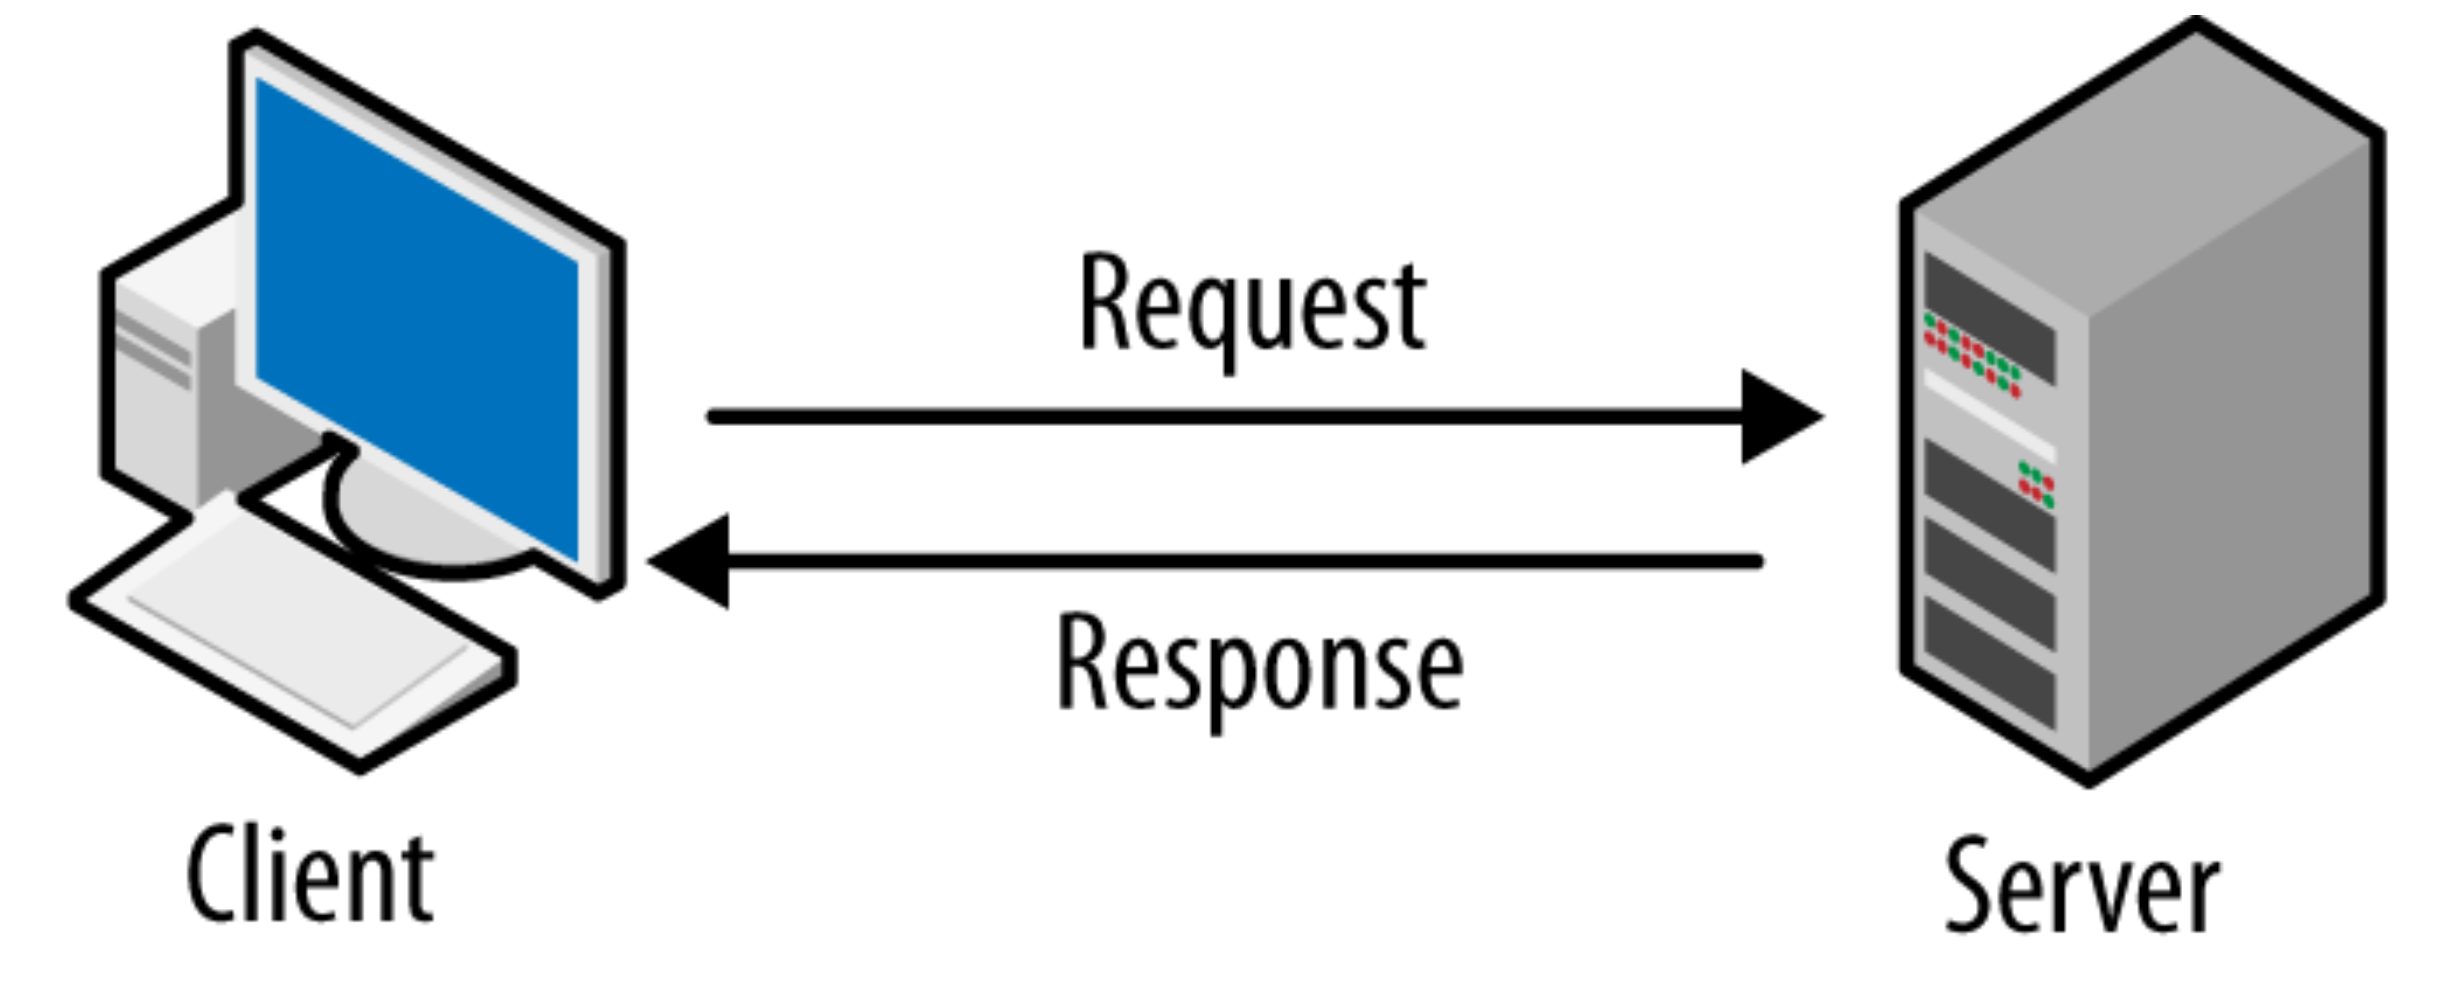
\includegraphics[width=10cm]{kepek/client_server_arch.png}
	\caption{A kliens-szerver, másnéven two-tier architektúra} %két szintű
	% https://madooei.github.io/cs421_sp20_homepage/assets/client-server-1.png
\end{figure}

Ebben az esetben a kliens megjeleníti a felhasználói interfészt, az interakció után pedig kérést küld a szervernek, majd az onnan kapott választ megjeleníti.
A szerver passzív szerepet tölt be, várja a kliensek kéréseit, melyeket teljesít és visszaküldi nekik a választ.

Ennek a felépítésnek az előnyei közé tartozik, hogy nagyon könnyen skálázható újabb szerverek és kliensek beiktatásával, illetve azáltal, hogy minden adat a szerveren tárolódik (\emph{centralizált adattárolás}), sokkal \emph{biztonságosabb} is, mert szabályozható az egyes erőforrásokhoz való hozzáférés.

Hátrányok közé sorolható, hogy ehhez gyakran elég drága szervereket kell vásárolni, illetve azok karbantartásához szakemberekre is szükség van. Ha a szerver meghibásodik, akkor annak javításáig, illetve cseréléséig senki sem tudja használni azt.

A fenti architektúrát egy újabb köztes réteggel bővítve három szintű (angolul three-tier), ennél több rétegnél pedig n rétegű (angolul n-tier) architektúrának nevezzük.

\begin{figure}[!ht]
	\centering
	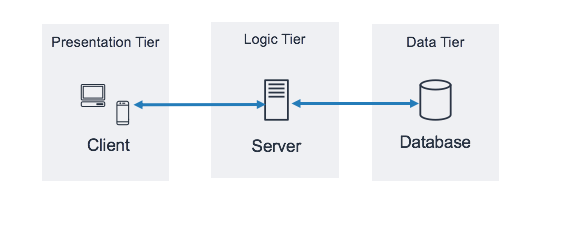
\includegraphics[width=12cm]{kepek/three_tier_arch.png}
	\caption{A háromrétegű architektúra}
	% https://docs.aws.amazon.com/whitepapers/latest/serverless-multi-tier-architectures-api-gateway-lambda/images/image2.png
\end{figure}

A háromrétegű architektúrában megkülönböztetjük a megjelenítési (angolul presentation), üzleti logika (angolul business logic), és perzisztencia (angolul data) rétegeket.

A megjelenítési réteg közvetlenül elérhető a felhasználó számára, mely a szervertől kapott adatoknak biztosít grafikus interfészt. Ehhez használatos a HTML leírónyelv, CSS stílusok és egyes esetekben a JavaScript, amely segítségével dinamikussá és lényegesen interaktívabbá tehető a felület.

Az üzleti logika rétegben található az alkalmazáshoz szükséges összes üzleti logika, hidat alkotva a kliens és az adatbázis között. A kliensektől érkező kéréseket fogadja, kiértékel, logikai döntéseket hoz, adatokat dolgoz fel, számolási feladatokat lát el.

Az adatbázis réteg feladata az adattárolás, és adathozzáférés biztosítása, melyet általában egy relációsadatbázis-kezelő rendszer (RDBMS) végez, mint például \emph{Oracle}, \emph{MySQL}, \emph{PostgreSQL}.
\chapter{Felhasznált technológiák ismertetése}

%\begin{megjegyzes}
%Megjegyzés szövege.
%\end{megjegyzes}

\chapter{Specifikáció}
% \cite[102.~oldal]{Fazekas}
% \cite{Fazekas,Tomacs}

\chapter{Fejlesztői dokumentáció}
% \cite[102.~oldal]{Fazekas}

\chapter{Összefoglalás}

\begin{thebibliography}{2}
	\bibitem{Fazekas}
	\textsc{Fazekas István}: \emph{Valószínűségszámítás}, Debreceni Egyetem, Debrecen, 2004.
	\bibitem{Tomacs}
	\textsc{Tómács Tibor}: \emph{A valószínűségszámítás alapjai}, Líceum Kiadó, Eger, 2005.
\end{thebibliography}
\end{document}